% I would rather have a bit of space between paragraphs
\setlength{\parskip}{0.5\baselineskip}

% I would like to include the abstract at the top
\begin{quote}
\small
\articleABSTRACT
\end{quote}


\section{Introduction}

\citet{lamichhane2003} described a Bayesian statistical method for
estimating the number and identity of essential genes in a genome from
data that indicates viable mutants. The genome of \emph{Mycobacterium
tuberculosis\/} was mutagenized with a transposon that inserted at
known sites, and a library of viable mutants was characterized. If a
mutant with insertion that disrupted a particular gene was viable,
that gene was indicated to be non-essential. Essential genes are those
for which no disruptive mutation could be viable.

The analysis method, described in further detail in
\citet{blades2002}, sought to estimate the overall proportion of
essential genes, and the probability that a gene was essential. We
assumed a uniform prior distribution on the number of essential genes,
and that genes were equally likely to be essential, and used Markov
chain Monte Carlo to derive the posterior probabilities of genes being
essential.

As part of the ReScience Ten Years Reproducibility Challenge, I sought
to reproduce the analysis in the paper, which I conducted in 2002
while an assistant professor in the Department of Biostatistics at
Johns Hopkins University. The bulk of the data and code were quickly
identified. (I keep collaborative projects in a directory
\verb|~/Projects| and save old projects in compressed form in
\verb|~/Projects/Tar|, and I immediately found
the file \verb|Gyanu.tgz|. Gyanu Lamichhane was first author on the
paper.) However, there were a number of challenges in reconstructing
the analysis steps, and the code used to conduct the computer
simulations underlying Figure~3 of \citet{lamichhane2003} appears
lost; I found only the results and the code to generate the figure.

The method was implemented in a combination of R \citep{R} and C
\citep{C} and assembled as an R package, R/negenes \citep{negenes},
which is available on both
\href{https://github.com/kbroman/negenes}{GitHub} and the
\href{https://cran.r-project.org/package=negenes}{Comprehensive R
  Archive Network (CRAN)}. The software used for the analyses in the
paper are a set of R scripts, along with one Perl script
\citep{Perl} that extracted transposon insertion sites from the \emph{M.
tuberculosis\/} genome.

\section{Challenges}

The first challenge in reproducing the analyses
in \citet{lamichhane2003} was to identify exactly what analyses needed
to be reproduced. The project directory did not contain any
documentation, and the file organization (Figure~\ref{fig:files}) was
quirky and contained a number of ancillary analyses that did not end
up in the paper. And so I had to resort to actually reading the
original article.



\begin{figure}
\definecolor{offwhite}{RGB}{255,250,240}
\lstset{language=bash,
        basicstyle=\ttfamily\scriptsize,
        frame=single,
        commentstyle=,
        backgroundcolor=\color{offwhite},
        showspaces=false,
        showstringspaces=false
        }

\begin{lstlisting}
class_problems.txt        findTA.pl*        Randomness/
Converge/                 mindGaps.pl*      Rawdata/
crucial_doubleTA.txt      Nov02/            Sept02/
Data/                     Operons/          Sims/
doubleta_hit.txt          R/                TroubleShootingSubClasses.txt
exploreSeq.pl*
\end{lstlisting}

\caption{Project directory for the work\label{fig:files}}
\end{figure}



There was some system behind the organization of the project files,
but it would have benefited from a \verb|ReadMe| file that
explained the structure. The
subdirectories \verb|Converge|, \verb|Operons|, \verb|Randomness|,
and \verb|Sims| contain the ancillary analyses that did not end up in the
paper. \verb|Rawdata| contains the primary data files, \verb|Data|
contains derived data files, and \verb|R| contains analysis scripts.

But actually \verb|Rawdata|, \verb|Data|, and \verb|R| contain files
for an initial analysis of the data performed in July, 2002. The subdirectory
\verb|Sept02| contains copies of those data and scripts
for a revised analysis performed in September, 2002; many of the files
are identicial, but additional data had been added.
Similarly, \verb|Nov02| contains further copies of the data and
scripts for a further revised analysis performed in November, 2002.

The bulk of the results in the paper are those from \verb|Nov02|.
Table~2 in \citet{lamichhane2003} includes results from \verb|Sept02|
as well as \verb|Nov02|. This was the primary challenge in reproducing
the analyses: identifying which versions of the analysis
scripts were used.

There were a number of further challenges in reproducing the results.
The code to produce Figure~1b in \citet{lamichhane2003} (see
Figure~\ref{fig:fig1b}, below) was not
present in the project directory, but rather was found in a separate
directory, with files for a talk that I gave on the work.

Further, the key analyses involved Markov chain Monte Carlo (MCMC),
but I had not saved the seeds for the random number generator, and so
I am not able to reproduce the results exactly. Also, I did not save
the key intermediate results to files, and I did not indicate which
objects were produced by which scripts. Rather, I left objects in the
R environment (saved in a \verb|.RData| file and re-loaded when R was
invoked) and used them as needed without explaining where they had
come from. Nevertheless, the analysis scripts were reasonably well
named (\verb|prepareData.R|, \verb|analysis.R|,
and \verb|figs4paper.R|), and so the order of the analysis could be
reconstructed without much difficulty.

\section{Code modifications}

Original analysis with R version 1.5.1 (2002-06-17)
latest with R version 3.6.1 (2019-07-05).

- table() and the need for as.numeric()

- small changes regarding cutoffs of what results were shown in two
  key tables



\section{The R/negenes package}

Talk about maintenance and changes of the R package.

- package placed on CRAN in ***. Changelog file indicates that this
  version of the package is from 2002-08-10, and so would be the one
  used for the analyses in the paper

- didn't start using version control until ***.

- Only substantive change was to fix a bug regarding over-running of
  array, identified by CRAN maintainers (give the date)

- various maintenance changes related to changing policies for R
  packages: for example, NAMESPACE file, registration of compiled code
  routines. Also changed the documetation to use
  Roxygen2 \citep{roxygen2}.




\section{Results}


\begin{figure}
\includegraphics[viewport=133 224 464 528, width=0.50\textwidth]{../original/Nov02/R/Figs/fig1.ps}
\hfill
\includegraphics[viewport=133 224 464 528, width=0.50\textwidth]{../reproduction/Figs/fig1.ps}

\caption{Figure 1a in Lamichhane et al. (2003). Original on left. Reproduction on right.\label{fig:fig1a}}
\end{figure}

\begin{figure}
\includegraphics[viewport=179 299 438 517, width=0.50\textwidth]{../talk/Figs/circlefig.ps}
\hfill
\includegraphics[viewport=179 299 438 517, width=0.50\textwidth]{../reproduction/Figs/circlefig.ps}

\caption{Figure 1b in Lamichhane et al. (2003). Original on left. Reproduction on right.\label{fig:fig1b}}
\end{figure}

\begin{figure}
\includegraphics[viewport=44 245 525 508, width=0.50\textwidth]{../original/Nov02/R/Figs/fig2.ps}
\hfill
\includegraphics[viewport=44 245 525 508, width=0.50\textwidth]{../reproduction/Figs/fig2.ps}

\caption{Figure 2 in Lamichhane et al. (2003). Original on left. Reproduction on right.\label{fig:fig2}}
\end{figure}


\section{Lessons}
